81. $\cfrac{(6-x-x^2)\sqrt{x-1}}{x-3}\geqslant0\Leftrightarrow\cfrac{(2-x)(x+3)\sqrt{x-1}}{x-3}\geqslant0.$ Применив метод интервалов, найдём ответ: $x\in\{1\}\cup[2;3).$
\begin{figure}[ht!]
\center{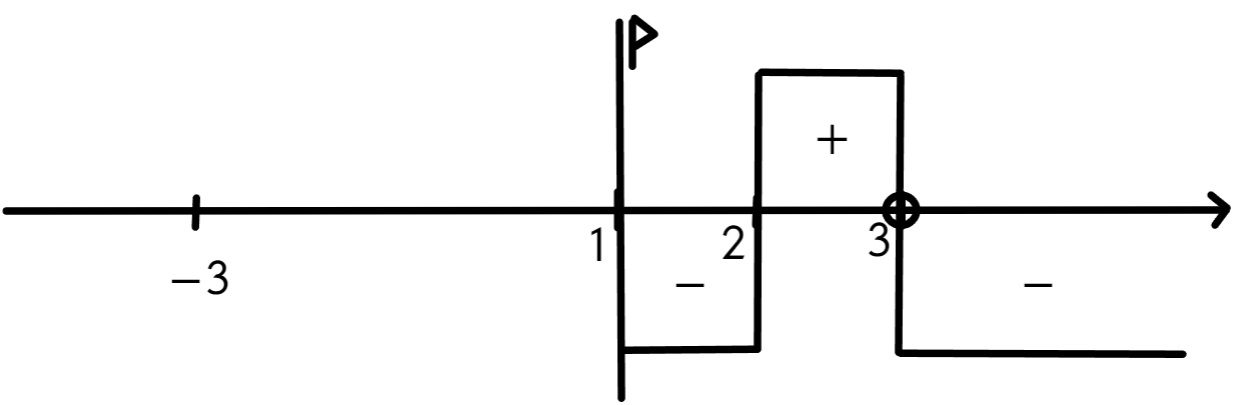
\includegraphics[scale=0.35]{ner9-82.png}}
\end{figure}\newpage\noindent
